\documentclass[11pt, a4paper]{IEEEtran}

\usepackage[T1]{fontenc}
\usepackage[utf8]{inputenc}
\DeclareUnicodeCharacter{21B3}{$\rightarrow$}

\usepackage[english]{babel}

\usepackage{tikz}
\usetikzlibrary{positioning,decorations.pathreplacing}
\usetikzlibrary{calc}

\usepackage{biblatex}
\addbibresource{rendu.bib}

\usepackage{authblk}


\usepackage{csquotes}
\usepackage{hyperref}
\usepackage{url}
\usepackage{listings}
\lstset{literate={↳}{$\rightarrow$}1}

\title{Reverse Engineering PlayReady CDM for EME}
\date{2023}
\author{Jules TIMMERMAN, \and Mohamed SABT\\SPICY, IRISA}


\begin{document}
\maketitle

\section{Introduction}

In 2022, the online video streaming industry was worth around 445 billion USD~\cite{business} and is still growing tremendously. Online platforms need to protect their content, usually using cryptography. They encrypt their content (usually videos and musics) using a key they store. They send this secret decryption key to authenticated users that were granted access to said content, usually through a subscription, an online purchase or a rental. Streaming services also need to limit access to the resource once the key was acquired: users should only be able to view the video for the period they were allowed. They should not be able to export it or watch it after their subscription has ended. This is what a Digital Right Management (DRM) system ensures.

Many big companies made their own DRM technologies such as Google's Widevine~\cite{widevine}, Microsoft's PlayReady~\cite{playready} and Apple's FairPlay~\cite{fairplay}. But DRM technologies work differently from one another with no common ground. Streaming platforms needed a common interface to be able to use the Web as a way to provide their content. With HTML5 native media playback support, the W3C created in 2012 along Netflix, Google and Microsoft, the Encrypted Media Extension (EME)~\cite{EME}. This specification created a common JavaScript interface to use DRMs on the web, without the need of plugins. Additionally, browsers do not have to implement an actual DRM themselves: they only have to call existing Content Decryption Modules (CDMs) on the user's device, that is, to redirect the function calls to the actual CDM function. EME was a step toward DRM interoperability on the Web.

There are many concerns and controversies that rose with EME. Many are due to EME not allowing open-source browsers to implement DRM support as they would need to rely on proprietary code, making DRM interoperability harder for newer and/or smaller browsers~\cite{effobjection}. It would also mean that the service is the one controlling your computer. This is what "Trusted Computing", sometimes dubbed "Treacherous Computing", is. Other issues are privacy concerns. Indeed, because the License Server (LS) needs information to identify your device, some of these information might be used in a malicious way to track your browser. Additionally, DRMs can be used to fingerprint your browser and identify your device by checking which configurations are supported. This has already been used on Reddit's website~\cite{reddit}. 

Because DRMs rely on closed source software, reverse engineering becomes the first step in studying it, whether it is for a security or a privacy research. Some DRMs have already been studied like Google's Widevine~\cite{widevinefunandprofit,wideleak}, but some were not closely examined. We plan on investigating PlayReady, in particular the content of the EME messages and how the actual CDM binary works. We also studied potential privacy issues related to PlayReady Test Server. Finally, we examined how licenses were encoded. 


\section{Background}

\subsection{Digital Right Management Technology}

A Digital Right Management (DRM) system is a technology that enables companies to provide access to media content, be it music, video, books or software, while protecting their content against piracy and enforcing rules to abide by to the user's device. A DRM system is characterized by two main components: the \emph{License Server} (LS) and the \emph{Content Decryption Module} (CDM). We call this pair a Key System. The CDM is the part responsible for enforcing the rules and decrypting content on the local device. The LS on the other hand, is the entity responsible for providing licenses to the user, so it can consume the content. A license in the context of DRMs is the decryption key (also called Content Key) used to read the content as well as the restrictions and rights associated with said key. There exist different restrictions, allowing many business models. The most common restrictions are time restrictions, granting access to video for only a certain amount of time, requiring that you ask the LS for a new license (or a renewal) if you want to watch the content after it expires.

There are other components that have a role in the DRM ecosystem. Usually, there is the Content Delivery Network (CDN) server that is used by users to get the encrypted videos. There is also the particular application a user is trying to use. This server is the one responsible for user authentication and is the main interface the user directly interacts with. 


\subsection{Microsoft PlayReady}

PlayReady is a DRM created by Microsoft in 2008~\cite{playready}. It is mostly present in Windows 10+ in the browser Edge. PlayReady has three different security levels that can be enforced in the license~\cite{sl}:
\begin{itemize}
	\item SL150: this level is the weakest and should only be used for testing as there is no actual protection.
	\item SL2000: this is the basic level to be used for commercial use. Secrets are protected according to the Compliance and Robustness Rules~\cite{compliancerobustness}. 
	\item SL3000: this is the highest level to date. It relies on hardware protection to keep data secrets.
\end{itemize}

In addition to the CDN and LS, PlayReady offers four optional servers:
\begin{itemize}
	\item Secure Stop Server~\cite{securestop}: handles the detection of when a user stops playback. It allows for a service to count how many users from the same account are watching a particular content and limit concurrent access.
	\item Secure Delete Server~\cite{securedelete}: ensures the deletion of a particular license that was stored on a client.
	\item Metering Server~\cite{metering}: measures user consumption (duration of a playback, episodes watched...)
	\item Domain Server~\cite{domain}:  manages user domains of the application. A domain is a group of users which are granted access to similar resources by sharing common decryption keys without the need of communicating with the license server.
\end{itemize}

\subsection{Encrypted Media Extension}

\subsubsection{Components}

The Encrypted Media Extension (EME) is a specification created by the W3C to allow the usage of DRM protection without any additional plugins~\cite{EME}. It introduces several JavaScript functions that can be used by webpages to interact with a CDM installed on the user machine. A simplified graphical explanation of DRM components related to EME can be found in figure \ref{fig:emecomp}.

\begin{figure}[h!]
	\centering
	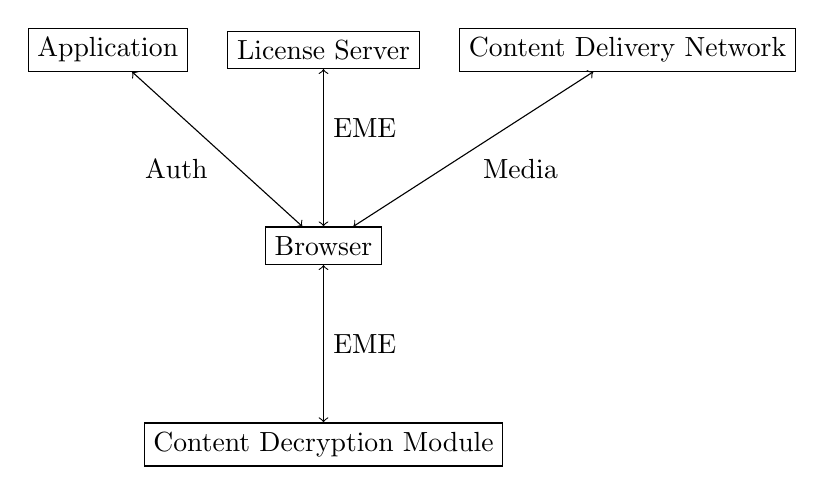
\begin{tikzpicture}[node distance=2cm and 0.5cm]
		\node[draw] (app) {Application};
		\node[draw, right=of {app}] (ls) {License Server};
		\node[draw, right=of {ls}] (cdn) {Content Delivery Network};

		\node[draw, below=of {ls}] (browser) {Browser};
		
		\node[draw, below=of {browser}] (cdm) {Content Decryption Module};
		
		\draw[<->] (app) -- node[below left] {Auth} (browser);
		\draw[<->] (ls) -- node[above right] {EME} (browser);
		\draw[<->] (cdn) -- node[below right] {Media} (browser);

		\draw[<->] (browser) -- node[right] {EME} (cdm);
	\end{tikzpicture}
	\caption{Summary of DRM Components}
	\label{fig:emecomp}
\end{figure}


\subsubsection{Workflow} \label{workflow}

We can describe a typical EME workflow as follows: 
\begin{enumerate}
	\item \texttt{requestMediaKeySystemAccess}: the script specifies a collection of Key Systems and configurations to try.
	\item \texttt{createMediaKeys}: gives access to the specified CDM
	\item \texttt{createSession}: creates a particular instance in the CDM. This marks the end of the initialization phase, and we can now use licenses
	\item \texttt{generateRequest}: creates the request to be sent to the LS. Initialization data has to be specified. It is usually given by inspecting the encrypted video we are trying to watch (via the \texttt{encrypted} event).
	\item \texttt{message} event: this event is raised whenever the CDM needs to send a message to the LS. The browser then generates the HTTP request with the specified body.
	\item \texttt{update}: this method has to be called with the response from the LS to the CDM.
\end{enumerate}
We can then loop the last three steps to ask for multiple licenses.

A summary of the workflow can be found in figure \ref{fig:emeworkflow}


\begin{figure}[h!]
	\centering
	\newcommand{\xdiff}{4} 			% Diff entre 2 colonnes
	\newcommand{\ydiff}{1.5}		% Diff verticale entre requêtes
	\newcommand{\responsediff}{0.2}	% Petite flèche de réponse
	\newcommand{\yheight}{7}
	\begin{tikzpicture}
		\node[draw] (browser) at (0,0) {Browser};
		\node[draw] (cdm) at (\xdiff,0) {CDM};
		\node[draw] (ls) at (-\xdiff,0) {LS};

		\draw (browser) -- ++(0, -\yheight);
		\draw (ls) -- ++(0, -\yheight);
		\draw (cdm) -- ++(0, -\yheight);

		\draw[->] (browser)++(0,-\ydiff) -- node[above, align=center] {\small\texttt{requestMediaKey}\\\texttt{SystemAccess}} ++(\xdiff,0);
		\draw[<-] (browser)++(0,-\ydiff-\responsediff) -- ++(\xdiff,0);

		\draw[->] (browser)++(0,-2*\ydiff) -- node[above] {\small\texttt{createMediaKeys}} ++(\xdiff,0);
		\draw[<-] (browser)++(0,-2*\ydiff-\responsediff) -- ++(\xdiff,0);

		\draw[->] (browser)++(0,-3*\ydiff) -- node[above] {\small\texttt{createSession}} ++(\xdiff,0);
		\draw[<-] (browser)++(0,-3*\ydiff-\responsediff) -- ++(\xdiff,0);

		\draw[->] (browser)++(0,-4*\ydiff) -- node[above] {\small\texttt{generateRequest}} ++(\xdiff,0);
		\draw[<-] (browser)++(0,-4*\ydiff-\responsediff) -- ++(\xdiff,0);
		\draw[->] (browser)++(0,-4*\ydiff-2*\responsediff) -- node[above] {\texttt{message} event} ++(-\xdiff,0);
		\draw[<-] (browser)++(0,-4*\ydiff-3*\responsediff) -- node[below] {License Response} ++(-\xdiff,0);
		\draw[->] (browser)++(0,-4*\ydiff-4*\responsediff) -- node[above] {\small\texttt{update}} ++(\xdiff,0);
	\end{tikzpicture} 
	\caption{Typical EME workflow}
	\label{fig:emeworkflow}
\end{figure}

\subsubsection{Privacy and EME}

The EME specification~\cite{EME} mentions Distinctive Identifiers and Distinctive Permanent Identifiers. It is defined as follows:
\begin{itemize}
	\item Distinctive Identifier: piece of data or observable behavior shared by only a small subset of individuals. This identifier is supposed to be clearable.
	\item Distinctive Permanent Identifier: A Distinctive Identifier which cannot be cleared, or is non-trivial to remove. Hardware-based identifiers are an example.
\end{itemize}

When requesting access to the Key System using \texttt{requestMediaKeySystemAccess}, you can specify in the configuration if Distinctive Identifiers can be used. It is up to the CDM to decide whether it will use some. A configuration will not be supported if it requires Distinctive Identifiers but the CDM refuses. These identifiers can be used to collect information about the client. As such, the EME specification~\cite{EME} recommends limiting or completely avoiding the use of these identifiers. When used outside the client, the identifiers must be encrypted. In general, EME puts forward a per-origin policy, as well as a per-browsing profile policy (like a user session) for identifiers.

In privacy, when investigating whether some data could be used maliciously, we usually investigate two properties: 
\begin{itemize}
	\item \emph{Uniqueness}: this indicates how many users share this value, and if it can be used to identify someone. Ideally (for fingerprinting), the value is unique per user and shared across origin but if only a handful shares it, it can still be used. 
	\item \emph{Stability}: this shows how often the value changes. The data is said to be stable when it rarely changes over time. 
\end{itemize}


\section{Contribution}

\subsection{EME Messages}

In a typical EME workflow as explained in section \ref{workflow}, EME messages are sent from the CDM to the LS and vice-versa while passing through the browser in events. We can observe EME functions using a plugin like EME Logger\footnote{Slightly modified version with hex dumps: \url{https://github.com/Avalonswanderer/wideXtractor/tree/main/eme_logger_widextractor}}. 
It allows us to see EME calls, their parameters, their return values and triggered events. In combination with the PlayReady (partial) documentation~\cite{playreadydoc} (the whole documentation is only available to PlayReady licensees), we can begin analyzing the opaque messages that are sent.

For the first tests, we used the Bitmovin Stream Test\footnote{\url{https://bitmovin.com/demos/stream-test}}, in combination with the Microsoft PlayReady Test Server\footnote{\url{https://testweb.playready.microsoft.com/}} as a license server.

\subsubsection{Initialization}

During the first three calls to the EME API, we can mostly see the configurations used by the platform in question, along the key used to identify the PlayReady Key System. Most notably, the session is temporary, that is, non-persistent and stored in-memory instead of on the hard drive. Distinctive identifier are not allowed. Audio and Video capabilities are also specified in the configuration as mentioned in the EME specification~\cite{EME}. 

\subsubsection{License Acquisition}

When requesting a license using the \texttt{generateRequest} call, we have to supply initialization data, as well as the type of said initialization data (usually "cenc" as in Common Encryption Standard~\cite{cenc}) used by the CDM to determine what licenses it needs. These variables are often supplied by the \texttt{encrypted} event that is triggered when playback is initiated on a DRM-protected video. In the case of PlayReady, the initialization data is the header of the file, called a PlayReady Header. This header uses the Simple Object Access Protocol (SOAP) format, which is derived from XML, making the content human-readable. It contains the Key ID (KID) that uniquely identifies the content we are trying to decrypt, as well as other information like the License Server URL or the used encryption method.

Once the CDM has processed the request, it will trigger a \texttt{message} event. The content of the message should then be forwarded to the license server by the JavaScript with a POST request. The message also uses the SOAP format. It contains the aforementioned PlayReady Header, as well as other data such as a License Nonce made to counter-act replay attacks, a digital signature and, most importantly, a field called Encrypted Data. It has two subfields : EncryptedKey and CipherValue. This data contains the private client information that is used by the LS to identify the user and send a license using their encrypted ECC Public Key. This key is encrypted using a key called WMRMServer, shared with the License Server. In addition, the license request message is signed using ECDSA. We summarize the different fields and the encryption used in Figure \ref{fig:licenserequest} and Figure \ref{fig:messagecrypto}. An example license request is shown in Appendix \ref{appendix:licenserequest}.

\begin{figure}
	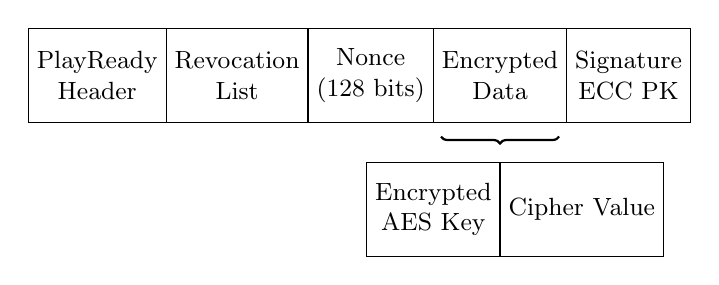
\begin{tikzpicture}[minimum height=1.2cm]
		\small;
		\node[draw,outer sep=0pt,align=center] (header) {PlayReady\\Header};
		\node[draw,anchor=west,outer sep=0pt,align=center] (revlist) at (header.east) {Revocation\\List};
		\node[draw,anchor=west,outer sep=0pt,align=center] (nonce) at (revlist.east) {Nonce\\(128 bits)};
		\node[draw,anchor=west,outer sep=0pt,align=center] (encdata) at (nonce.east) {Encrypted\\Data};
		\node[draw,anchor=west,outer sep=0pt,align=center] (sig) at (encdata.east) {Signature\\ECC PK};

		\draw[decorate,thick,decoration={brace,mirror,raise=5pt}] ($(encdata.south) + (-0.75,0)$) -- ($(encdata.south)+ (0.75,0)$);

		\node[draw,anchor=north east,outer sep=0pt,align=center] (enckey) at ($(encdata.south)+ (0,-0.5)$) {Encrypted\\AES Key};
		\node[draw,anchor=west,outer sep=0pt,align=center] (ciphervalue) at (enckey.east) {Cipher Value};

	\end{tikzpicture}

	\caption{Fields present in a license request message}
	\label{fig:licenserequest}
\end{figure}

\begin{figure}[h!]
	\newcommand{\xdiff}{-5.5} 		% Diff entre 2 colonnes
	\newcommand{\ydiff}{3}			% Diff entre 2 lignes
	\newcommand{\xdiffd}{\xdiff/2}	% Division par 2 des commandes
	\newcommand{\ydiffd}{\ydiff/2}
	\begin{tikzpicture}
		\node[align=center] (ECCPK) at (0, \ydiffd) {Client Information\\(Device ECC PK)};
		\node[draw,align=center] (aescbc) at (0,0) {AES 128\\CBC};
		\node[draw,align=center] (ecc256) at (\xdiffd,\ydiffd) {ECC 256\\ElGamal};
		\node[align=center] (encAESkey) at (\xdiffd, 0) {Encrypted\\AES Key};
		\node[align=center] (WMRMServer) at ($(ecc256) + (\xdiffd,0)$) {WMRMServer\\Key};
		\node[align=center] (AESkey) at ($(ecc256) + (0,\ydiffd)$) {AES Key};
		\node[align=center] (encECCPK) at (0,-\ydiffd) {Cipher Value};

		\draw[->] (AESkey) -- (ecc256);
		\draw[->] (WMRMServer) -- (ecc256);

		\draw[->] (ecc256) -- (encAESkey);
		\draw[->] (encAESkey) -- (aescbc);
		\draw[->] (ECCPK) -- (aescbc);

		\draw[->] (aescbc) -- (encECCPK);
	\end{tikzpicture}

	\caption{Cryptographic functions used in a license request}
	\label{fig:messagecrypto}
\end{figure} 

After the message is sent, we listen for the response of the LS. We can then feed the response directly to the CDM with the \texttt{update} function. The license is now available and playback can be started.


\subsection{PlayReady Test Server}

\subsubsection{Test Server}

Microsoft has created a PlayReady test server that can be used by app developers (even non-licensees) to test how their product works by requesting licenses with custom rights. Some content is available on the platform, but you can also test your own content by specifying content keys and KID. Among all the policies you can ask for in a license, you can specify start and end dates for the license, the minimum security level and whether the license is persistent. The rights and restrictions requested are encoded in the URL query.

Most interestingly, the test server has an option called \texttt{clientinfo} which can be used to retrieve the private client information that were sent along the license acquisition request.

\subsubsection{Client Info} \label{sec:clientinfo}

This option is only available on the test server. It is supposed to act as a reflector for the client information that was sent. It is to be noted that the information is encrypted in the license request, making it sensitive information. An example of the response can be found in Appendix \ref{appendix:clientinfo}. The main information is the Client time and CDM version, the supported features and the digital certificate chain. 

We tried to investigate the different fields and whether they could be used for fingerprinting. As such, we studied two properties of the data: its uniqueness and its stability. More precisely, we focused on two values: \emph{Digest} Value of certificate 0 (the client certificate) and the \emph{Signature Public Key} of the client that was sent after generating the request. We tested on a few different machines using Windows 10 or Windows 11 and Microsoft Edge, as PlayReady was not available in other browsers and operating systems. To conduct the tests, we used a website that would print the client info and the signature public key\footnote{https://github.com/jules-timmerman/PlayReady-Reverse-Intern/tree/main/ClientInfoPoC}. This site doubled as a proof of concept of how the test server could be abused to collect information about a user: a malicious website could 
use JavaScript in the page and call the EME API with the PlayReady Test Server, without any visual effect (like a video) for the user. 

We found that the public key as well as the digest value were unique per device and stable (for a few weeks of testing). It is quite interesting that the digest value was changing from client to client when the content of the certificate that was displayed was not different. This would suggest that there were other information that we were not reflected. Furthermore, other fields reflected could be used to track and collect data about a user like the Platform (usually \texttt{Windowsx86}) or the Model Number, hinting toward a specific Windows version. In addition, some devices support hardware protection. It can be activated using a Key System allowing security level 3000\footnote{\texttt{com.microsoft.playready.recommendation.3000}}, the hardware security level. It shows a different platform related to the GPU (for example Nvidia or Intel) and another model number, further improving the quality of the fingerprint, while staying unique and stable.

On Microsoft Edge, DRMs are activated by default and no authorization is asked on a per-origin basis. This means that a script could run completely silently. On the other hand, the signature public key and the digest are unique per-origin, meaning a user cannot be tracked from one website to the other with this method as a new key and digest are generated for each origin. Moreover, Microsoft Edge provides an option to clear all data related to Media Foundation, meaning all data linked to the CDM, like persistent licenses, would be purged. It also has the effects of generating a new signature public key and digest. It also changes the values when using hardware protection, thus not giving any additional stability. Although the data can easily be cleared and changed, we had identical values when using a private session or the strict privacy mode from Edge. We did have different values when using a different browsing session. It makes PlayReady comply with EME.

\subsection{License Format}

Licenses follow the Extensible Media Rights (XMR) system. It is used to encode the policies  as well as the encrypted content key. While the specification of this format is only available to PlayReady licensees, we have a good idea of what information are stored in the license thanks to the PlayReady documentation~\cite{licenseacquisition,contentencryption}. It explains the used encryption methods as well as a few diagrams with the content of a license.


We used the PlayReady Test Server to sample many licenses that we would then compare to deduce the semantic of the fields. We used a script to automate the sampling phase\footnote{\url{https://github.com/jules-timmerman/PlayReady-Reverse-Intern/tree/main/LicenseComparison}}. It would try all possible combinations of the arguments and store the request. It also does multiple requests of the same license to help with finding random values.

The XMR format seems like it follows a construction akin to Tag-Length-Value. For each field, we have a value on three bytes that identifies the type of data that follows. We then have a length indicator on four bytes representing the combined size of the tag, length  and data (including the ending null byte) in bytes. It is followed by the data and terminated by a null byte. A summary of the fields we found are available in Appendix \ref{appendix:licensefields}. This analysis seems to match what had been done previously~\cite{securityexploration}, even though the toolchain developed is not available. There also seems to be a system of blocks, with some tags encapsulating other ones. 

There might be a better subdivision: for example, we might be able to split the tag or length in two, giving a separated semantic to each part. The previous analysis~\cite{securityexploration} seems to have done that separation but not additional meaning was given.

We observed three blocks of data that changed at every request, indicating a form of randomness. The first one was right after the XMR header of the license and represented the license Nonce. We then have a block of 1024 bits. It is the biggest encrypted block, so we believe it is where the Content Key is encrypted using ECC256 ElGamal~\cite{contentencryption}, with some additional information. We know that the Content Key is 128 bit long from the PlayReady documentation~\cite{contentencryption} and the PlayReady Header, hence the additional data. At the end of the license, we have a 128 bits block. It is the license MAC, called the license signature by PlayReady, generated using AES OMAC1.

Another block of interest is the one right after the Content Key. It seems to be a 512-bit key, unique per device and per origin. It is the same as the client info regarding its stability in different browsing contexts, as discussed in section \ref{sec:clientinfo}. In the Security Exploration example~\cite{securityexploration}, it was named \emph{ECC Device Key}. It does not seem to be linked to any cryptographic function we were able to observe so far. A summary can be found in Figure \ref{fig:licensefields}

\begin{figure}
	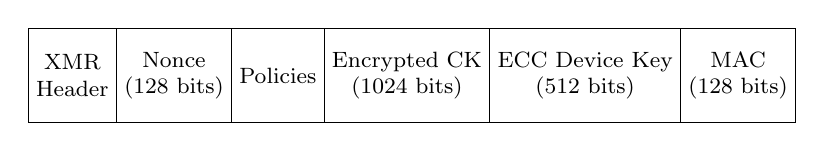
\begin{tikzpicture}[minimum height=1.2cm, anchor=west,outer sep=0pt,align=center]
		\footnotesize;
		\node[draw] (header) {XMR\\Header};
		\node[draw] (nonce) at (header.east) {Nonce\\(128 bits)};
		\node[draw] (policies) at (nonce.east) {Policies};
		\node[draw] (encCK) at (policies.east) {Encrypted CK\\(1024 bits)};
		\node[draw] (devicekey) at (encCK.east) {ECC Device Key\\(512 bits)};
		\node[draw] (mac) at (devicekey.east) {MAC\\(128 bits)};
	\end{tikzpicture}

	\caption{Fields present in a license}
	\label{fig:licensefields}
\end{figure}

\subsection{PlayReady on Windows}

\subsubsection{Samples}

We wanted to investigate the PlayReady binary used by Microsoft Edge. To work on a smaller project than Microsoft Edge, we found two samples created by Microsoft to showcase the usage of PlayReady: one using C++\footnote{\url{https://github.com/microsoft/media-foundation/tree/master/samples/MediaEngineEMEUWPSample}} and one using C\#\footnote{\url{https://github.com/microsoft/windows-universal-samples/tree/main/Samples/PlayReady}}. Both applications used the Universal Windows Platform (UWP) to leverage the Windows API. They use Media Foundation, Windows' API for media playback.

\subsubsection{Reversing the DLL library}

The C++ application uses a DLL\footnote{Called \texttt{Windows.MediaProtection.PlayReady.dll}} located in \texttt{System32}, Windows default directory for system libraries. This dynamic library shares the same name as the UWP namespace of PlayReady. We tried to reverse it with two different approaches: 
\begin{itemize}
	\item \emph{dynamically}, using the Visual Studio debugger
	\item \emph{statically}, using Ghidra, a static reversing tool.
\end{itemize}

The binary was stripped, meaning all symbols had been removed, making reversing harder. Our goal when reversing the DRM was to find precisely how the licenses were parsed. By looking at the strings in the binary, we could find some strings that were used in the license response. We tried to set a breakpoint in the binary to functions that used said strings, but it was not hit. It helped us notice a gap between the static disassembly of the functions and how they were loaded in memory: it seemed that the functions were constructed after the DLL was loaded in memory. We dumped the DLL from memory after it was loaded to recover the correct functions.

We were not able to understand the parsing done in the binary in our limited time as it was too time-consuming a task.


\section{Related Works}

This work is heavily related to the works that were investigating the inner-workings of Google's DRM, Widevine~\cite{wideleak,widevinefunandprofit}. Privacy issues and concerns are also raised in~\cite{drmcanwatchyoutoo}. In that paper, they found identifiers that were shared across origins, allowing for effective fingerprinting.



\section{Conclusion}

In this paper, we tried to investigate if PlayReady complied with EME, like it was done for other DRM technologies. While we did not find any particular identifiers that could be used across origins, the test server can still be abused to query for some components of the user system, like their OS versions or their GPU model. We would need to scale the tests we have done to be able to have a more precise idea on how unique some values can be. In addition to the privacy issues, our understanding of the license format can help to create tools to aid the investigation of PlayReady, like plugins automatically parsing licenses. Lastly, we did find the PlayReady binary and dumped it from memory. While we were not able to do much with it, it is still the first step to reverse it.


\section*{Bibliography}
\printbibliography


\newpage
\onecolumn
\begin{appendices}

\section{License Request} \label{appendix:licenserequest}

\lstset{tabsize=1}
\begin{lstlisting}[breaklines, caption={Sample License Request message},mathescape]
<PlayReadyKeyMessage type="LicenseAcquisition">
	<LicenseAcquisition Version="1">
		<Challenge encoding="base64encoded">
			<?xml version="1.0" encoding="utf-8"?>
				<soap:Envelope
					xmlns:xsi="http://www.w3.org/2001/XMLSchema-instance"
					xmlns:xsd="http://www.w3.org/2001/XMLSchema"
					xmlns:soap="http://schemas.xmlsoap.org/soap/envelope/">
					<soap:Body>
						<AcquireLicense
							xmlns="http://schemas.microsoft.com/DRM/2007/03/protocols">
							<challenge>
								<Challenge
									xmlns="http://schemas.microsoft.com/DRM/2007/03/protocols/messages">
									<LA
										xmlns="http://schemas.microsoft.com/DRM/2007/03/protocols" Id="SignedData" xml:space="preserve">
										<Version>1</Version>
										<ContentHeader>
											<WRMHEADER
												xmlns="http://schemas.microsoft.com/DRM/2007/03/PlayReadyHeader" version="4.0.0.0">
												<DATA>
													<PROTECTINFO>
														<KEYLEN>16</KEYLEN>
														<ALGID>AESCTR</ALGID>
													</PROTECTINFO>
													<KID>4Rplb+TbNES8tGkNFWTEHA==</KID>
													<CHECKSUM>KLj3QzQP/NA=</CHECKSUM>
													<LA_URL>https://profficialsite.keydelivery.mediaservices.windows.net/PlayReady/</LA_URL>
													<CUSTOMATTRIBUTES>
														<IIS_DRM_VERSION>8.1.2304.31</IIS_DRM_VERSION>
													</CUSTOMATTRIBUTES>
												</DATA>
											</WRMHEADER>
										</ContentHeader>
										<CLIENTINFO>
											<CLIENTVERSION>10.0.16384.10011</CLIENTVERSION>
										</CLIENTINFO>
										<RevocationLists>
											<RevListInfo>
												<ListID>ioydTlK2p0WXkWklprR5Hw==</ListID>
												<Version>11</Version>
											</RevListInfo>
											[...]
										</RevocationLists>
										<LicenseNonce>MKAsWyCrYniFmdE5MFuVVg==</LicenseNonce>
										<ClientTime>1685106075</ClientTime>
										<EncryptedData
											xmlns="http://www.w3.org/2001/04/xmlenc#" Type="http://www.w3.org/2001/04/xmlenc#Element">
											<EncryptionMethod Algorithm="http://www.w3.org/2001/04/xmlenc#aes128-cbc"></EncryptionMethod>
											<KeyInfo
												xmlns="http://www.w3.org/2000/09/xmldsig#">
												<EncryptedKey
													xmlns="http://www.w3.org/2001/04/xmlenc#">
													<EncryptionMethod Algorithm="http://schemas.microsoft.com/DRM/2007/03/protocols#ecc256"></EncryptionMethod>
													<KeyInfo
														xmlns="http://www.w3.org/2000/09/xmldsig#">
														<KeyName>WMRMServer</KeyName>
													</KeyInfo>
													<CipherData>
														<CipherValue>$\mathbf{base64 encoded}$</CipherValue>
													</CipherData>
												</EncryptedKey>
											</KeyInfo>
											<CipherData>
												<CipherValue>$\mathbf{base64 encoded}$</CipherValue>
											</CipherData>
										</EncryptedData>
									</LA>
									<Signature
										xmlns="http://www.w3.org/2000/09/xmldsig#">
										<SignedInfo
											xmlns="http://www.w3.org/2000/09/xmldsig#">
											<CanonicalizationMethod Algorithm="http://www.w3.org/TR/2001/REC-xml-c14n-20010315"></CanonicalizationMethod>
											<SignatureMethod Algorithm="http://schemas.microsoft.com/DRM/2007/03/protocols#ecdsa-sha256"></SignatureMethod>
											<Reference URI="#SignedData">
												<DigestMethod Algorithm="http://schemas.microsoft.com/DRM/2007/03/protocols#sha256"></DigestMethod>
												<DigestValue>$\mathbf{base64 encoded}$</DigestValue>
											</Reference>
										</SignedInfo>
										<SignatureValue>$\mathbf{base64 encoded}$</SignatureValue>
										<KeyInfo
											xmlns="http://www.w3.org/2000/09/xmldsig#">
											<KeyValue>
												<ECCKeyValue>
													<PublicKey>$\mathbf{base64 encoded}$</PublicKey>
												</ECCKeyValue>
											</KeyValue>
										</KeyInfo>
									</Signature>
								</Challenge>
							</challenge>
						</AcquireLicense>
					</soap:Body>
				</soap:Envelope>
		</Challenge>
		<HttpHeaders>
			<HttpHeader>
				<name>Content-Type</name>
				<value>text/xml; charset=utf-8</value>
			</HttpHeader>
			<HttpHeader>
				<name>SOAPAction</name>
				<value>"http://schemas.microsoft.com/DRM/2007/03/protocols/AcquireLicense"</value>
			</HttpHeader>
		</HttpHeaders>
	</LicenseAcquisition>
</PlayReadyKeyMessage> 

	
\end{lstlisting}

\pagebreak
\section{Client Information} \label{appendix:clientinfo}
\begin{lstlisting}[breaklines, caption={Client Information and Signature Key from a computer with an Nvidia 4070}]
Signature Public Key: x60jY9jVEIWph4Z3+Ow/7pwQRiDJuVZQSjiRJtmVqi+c0frm3QzF31lHgTFeBftZH4VzQLaa9TONew+E9w0wDg==

Client Info:

Client Version: 10.0.16384.10011
Client Time: 7/10/2023 5:35:46 PM

Supported Features:

RevocationLists
PlayReady3Features

Device Certificate Info (Cert 0):

Platform: OEM
Type: Device
SecurityLevel: 3000
RobustnessVersion: 16777216
ManufacturerName: Nvidia Corporation
ModelName: AD10X
ModelNumber: AD10X
DigestValue: dMGc6BzMMaVOWDaS03AADOzMrBffsS93dzWpB9g3fCE=
IssuerKey: fiNb/dkIy09gdm23dxS6nFHSrbvkDmLM0ZOCLZTndoekbPR+H5a2jvAGh36bqQkfbBg5x/2PdqPw/rTr5kuIUQ==

Certificate Chain:

↳ Cert: 1
ManufacturerName: Nvidia Corporation
ModelName: AD10X
ModelNumber: AD10X
DigestValue: l5Ri+OkuHnaW321J23bp4/vSrxVVdb84zprsEGTsgAw=
Platform: OEM

↳ Cert: 2
ManufacturerName: Nvidia Corporation
DigestValue: pFOP5LRTEEOsd/knDWcNnWU0jwoLzFRd9Z0byKwXmQA=

↳ Cert: 3
ManufacturerName: Microsoft
ModelName: PlayReady SL3000 Device Port + Link CA
ModelNumber: 1.0.0.1
DigestValue: bk7YOJRioSgnzjpZgLasowaL96LFIBHDx6B0z+JoDPE=
\end{lstlisting}

\pagebreak
\section{License policies} \label{appendix:licensefields}
\centering
\begin{tabular}{|c|c|p{10cm}|}
\hline
\emph{Tag} & \emph{Name} & \emph{Description}\\
\hline
\hline
0x010012 & Begin Date / End Date & Epoch time of when the license starts / expires\\
\hline
0x010030 & First Expiration & License will expire after that amount of second and playback will not be able to start again \\
\hline
0x010034 & Security Level & Minimum Security Level required by the license to allow playback\\
\hline
0x01000a & KID and CK & KID then the encrypted data with the Content Key, separated by 0x000100030080 (indicating 80 bytes long data)\\
\hline
0x00002a & ECC Device Key & Exact usage unknown (unique per client and origin)\\
\hline
0x01000b & Signature & License AES OMAC1 Signature\\
\hline

\end{tabular}



\end{appendices}


\end{document}